\newtheorem{definition}{Definition}[subsection]


\subsection{Markov Decision Processes}
\begin{definition}

A Markov Decision Process (MDP) is defined by its state and action sets and by the one-step dynamics of the environment \cite{RLAnIntro}. This is represented as a 4-tuple $(S, A_{s}, P, R)$, where
\begin{itemize}
  \item $S$ is a finite set of states,
  \item $A$ is a mapping from state $s$ to a set of actions,
  \item $P(s, a, s')$ is the probability that state $s$ will move to state $s'$when action $a$ is performed
  \item $R(s, a, s')$ is the immediate reward received after transitioning from state $s$ to $s'$, due to action $a$.
\end{itemize}

\end{definition}
$R$ is referred to as the \textit{reward function}.

\subsection{Reinforcement Learning}
Reinforcement Learning (RL) is a paradigm of Machine Learning (ML) that attempts to solve a specified MDP (usually by maximising the total accrued reward in some way or another). RL aims to generate a \textit{policy} $\pi : S \to A$, where $S$ is the set of states and $A$ is the set of possible actions (the policy may also take the form of a probability distributions, mapping a state-action pair to a probability). This policy is developed during the training phase, and then can be used to choose each action during execution.

RL algorithms can be either model-based or model-free. In model-based RL, the agent internally represents the environment in order to be able to predict subsequent states. In model-free RL the agent has no access to a model of the environment. Every RL algorithm discussed in this paper will be model-free.

In an RL algorithm we also specify a learning rate $\alpha$ and discount factor $\gamma \in [0,1]$. The learning rate specifies to what extent new information is prioritised over older information, so that with a learning rate of 0, the agent learns nothing new, but with a learning rate of 1, only the most recent experience is considered. The discount factor determines the importance of future rewards. A discount rate of 1 values a reward far in the future just as much as an immediate reward, but a discount factor of 0 only considers the immediate reward.



\subsection{Q-Learning}
The Q-learning algorithm maintains a state-action value function $Q : S \times A \to \mathbb{R}$ which specifies the quality of performing an action $a$ when in state $s$ and then following policy $\pi$. This value represents the discounted expected return of choosing action $a$ in state $s$. The algorithm typically gives the policy (which is independent of Q-learning) in accordance with the $\epsilon$-greedy action choice method:


\[ \pi(s) = \begin{cases} 
      \pi(s) = \text{action } a \sim U(A_s) & \text{with probability $\epsilon$} \\
      \argmax_{a \in A}Q(s,a) & otherwise                         
   \end{cases}
\]

Informally, a random action is chosen with probability $\epsilon$, and the best action (according to the $Q$-function) otherwise.

$Q$ is initialised to an arbitrary fixed value, usually $0$. At each timestep $t$, the algorithm chooses an action $a_t$ according to some policy. This action is then performed, moving from state $s_t$ to a new state $s_{t+1}$. The value of $Q(s_t,a_t)$ is then updated as follows:

\[Q^{\textit{new}}(s_t,a_t) = (1-\alpha) \cdot Q(s_t,a_t) + \alpha \cdot (r_t + \gamma \cdot \argmax_{a \in A}Q(s_{t+1},a))\]

where $\alpha$ is the learning rate and $\gamma$ is the discount factor.

The term $\argmax_{a \in A}Q(s_{t+1},a)$ is the estimate of the optimal accumulated future reward. We use bootstrapping from the current estimate of the value function, making this a \textit{temporal difference} algorithm \cite{RLAnIntro}.

In standard Q-learning, the $Q$ function is stored as a table (a \textit{Q-table}) with states as rows, and actions as columns. As the state or action space grows, the Q-table becomes too large to store, as the number of states is exponential in the number of state dimensions. This is referred to as the ``Curse of Dimensionality'' \cite{cod}. This leads to another approach of representing the function with the use of neural networks.


\subsection{Neural Networks}

Neural networks aim to approximate a mathematical function. The network consists of multiple layers of artificial neurons which linearly combine inputs and uses an \textit{activation function} (which is typically non-linear) to compute an output. The outputs of each neuron in a particular layer form the inputs of each neuron in the next layer. More formally, we represent the weights of a layer $l$ by matrix $\boldsymbol{W}^l$, so that for neuron $i$ in layer $l$, the weight of the input from neuron $j$ from layer $l-1$ is $\boldsymbol{W}^l_{ij}$. We represent the biases of layer $l$ by vector $\boldsymbol{b}^l$, so that for neuron $i$, the value $\boldsymbol{b}^l_i$ is added to the result of the linear operation. Therefore, we can define the activations of a layer $l$ \cite{csmlnotes}, $\boldsymbol{a}^{l}$:

\[
\boldsymbol{z}^l = \boldsymbol{W}^l \boldsymbol{a}^{l-1} + \boldsymbol{b}^l
\]
\[
\boldsymbol{a}^{l} = f(\boldsymbol{z}^{l})
\]
where $f$ is the non-linear activation function.

The input of the network is $\boldsymbol{a}^0 = \boldsymbol{x}$, and the output of the network is $\boldsymbol{y} = \boldsymbol{a}^L$, where $L$ is the number of layers.

A loss function is a mapping from a set of values to a real number in order to represent some intuitive ``cost''. To train the network, we alter the weights and biases in the direction specified by the gradient of this loss function with respect to the variable in question ($\boldsymbol{W}^l$ or $\boldsymbol{b}^l$). This is called the back-propagation algorithm. The back-propagation equations are given below \cite{csmlnotes}:

\[\frac{\partial \mathcal{L}}{\partial \boldsymbol{z}^L} =\frac{\partial \mathcal{L}}{\partial \boldsymbol{a}^L} \cdot \frac{\partial \boldsymbol{a}^L}{\partial \boldsymbol{z}^L}\]

\[\frac{\partial \mathcal{L}}{\partial \boldsymbol{z}^l} = \frac{\partial \mathcal{L}}{\partial \boldsymbol{z}^{l+1}} \boldsymbol{W}^{l+1} \frac{\partial \boldsymbol{a}^l}{\partial \boldsymbol{z}^{l}}\]

\[\frac{\partial \mathcal{L}}{\partial \boldsymbol{W}^l} = (\boldsymbol{a}^{l-1} \frac{\partial \mathcal{L}}{\partial \boldsymbol{z}^l} )^T\]

\[\frac{\partial \mathcal{L}}{\partial \boldsymbol{b}^l} =\frac{\partial \mathcal{L}}{\partial \boldsymbol{z}^l}\]



\subsubsection{Convolutional Neural Networks}
Convolution Neural Networks (CNNs) use a convolution operation: a linear operation in place of matrix multiplication found in standard neural networks \cite{cnn}. This convolution operation consists of a \textit{kernel} (a small tensor) that performs dot products over the input tensor in accordance with parameters such as stride and padding. The \textit{stride} of a convolution is how much the kernel moves between dot products, and \textit{padding} indicates how many layers of zeroes to add to the border of the input tensor \cite{cnn}. The convolution operation is illustrated in figure \ref{fig:cnn}.

\begin{figure}
    \centering
    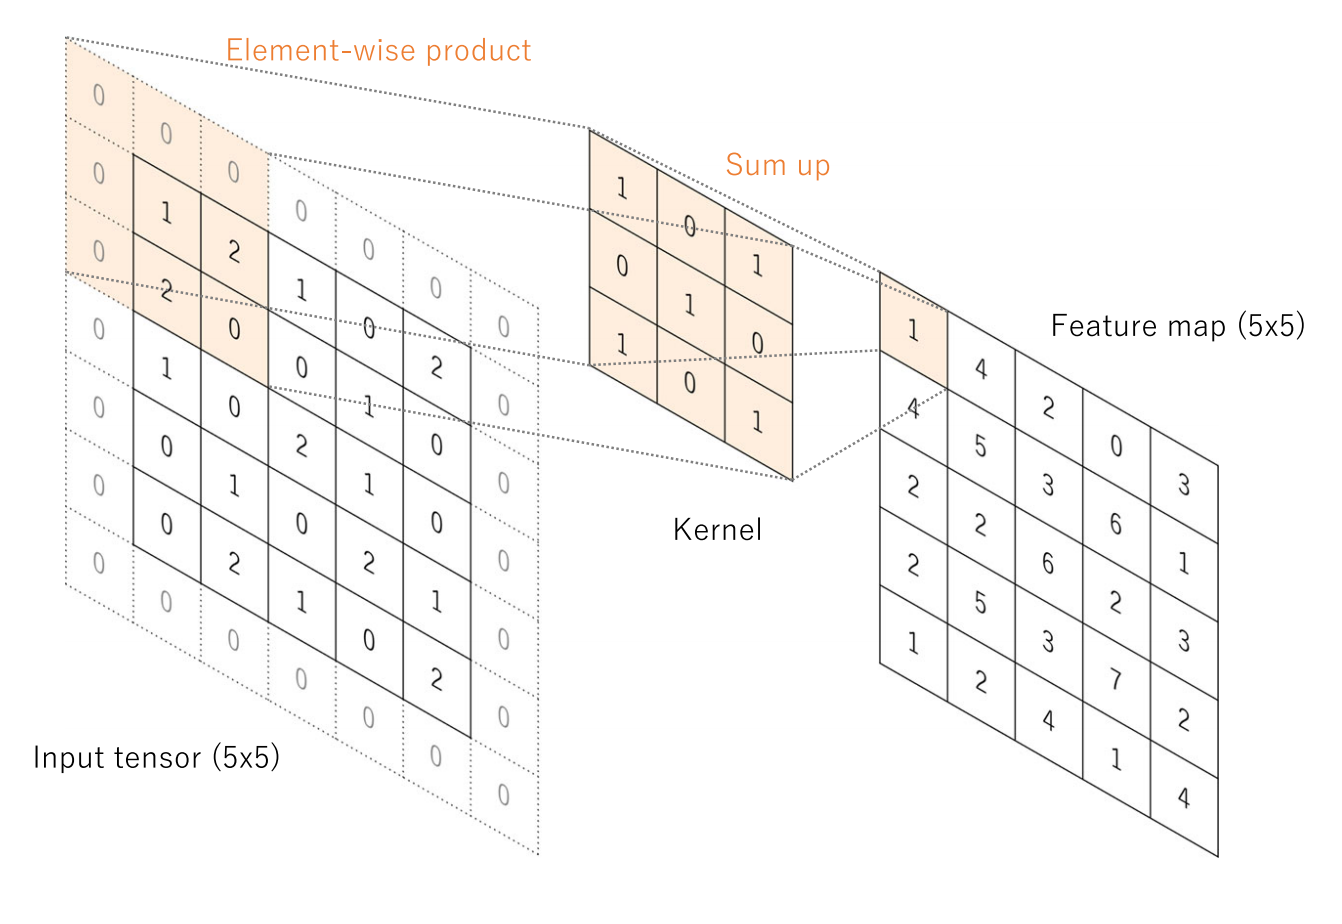
\includegraphics[scale = 0.25]{images/cnn.png}
    \caption{A convolution operation with zero padding so as to retain in-plane dimensions. Image and caption source: \cite{cnnfig}}.
    \label{fig:cnn}
\end{figure}

To make this more formal, consider this formalisation from \cite{csmlnotes}:

Suppose we apply $F_{l+1}$ filters, each of shape $W_f \times H_f \times F_t$, then we can write the entries $z_{i',j',f'}^{l+1}$ in this layer as follows (we assume no zero-padding and stride of 1 in each direction):



 \[z_{i',j',f'}^{l+1} = b^{l+1,f'} + \sum_{i=1}^{W_{f'}}\sum_{j=1}^{H_{f'}}\sum_{f=1}^{F_l}a^l_{i'+i-1,j'+j-1,f} w^{l+1,f'}_{i,j,f}
 \]
 
 Above $w^{l+1,f'}_{i,j,f}$ is the parameter for the $f$'th filter between layers $l$ and $l+1$ indexed by $(i,j,f)$ \cite{csmlnotes}.
 
 
 
Other operations, such as pooling, can be used in a CNN. \textit{pooling} refers to the idea of reducing the size of a tensor (usually after a convolutional layer) using a mathematical operation \cite{cnn}.

\subsubsection{Recurrent Neural Networks}
Recurrent Neural Networks (RNNs) are a class of neural network that is able to ``remember'' previous inputs using an internal state \cite{rnn}, allowing it to deal with sequential inputs (unlike a standard neural network which does not maintain an internal state). For long time-series data an RNN can suffer from the \textbf{vanishing gradient problem} \cite{rnn} which occurs when the gradient of the loss function approaches zero, thus reducing the changes made to weights and severely limits its ability to train. 

A solution for this problem in RNNs is to use a Gated Recurrent Unit (GRU) \cite{gru} which have operations update-gate and reset-gate which are used to filter the amount of passed information to consider. 

Another popular architecture is the LSTM \cite{lstm}, which is similar to the GRU architecture, but provides a forget gate, which regulates the amount of information to be ``forgotten'', and an output gate which decides on the next hidden state \cite{lstm}.

LSTMs and GRUs have both exhibited similar performance in natural language processing tasks \cite{lstmvsgru}, so we will only consider the use of GRU-cells in the architectures of this project.

Figure \ref{fig:rnn} shows the of the LSTM and GRU architectures.

\begin{figure}
    \centering
    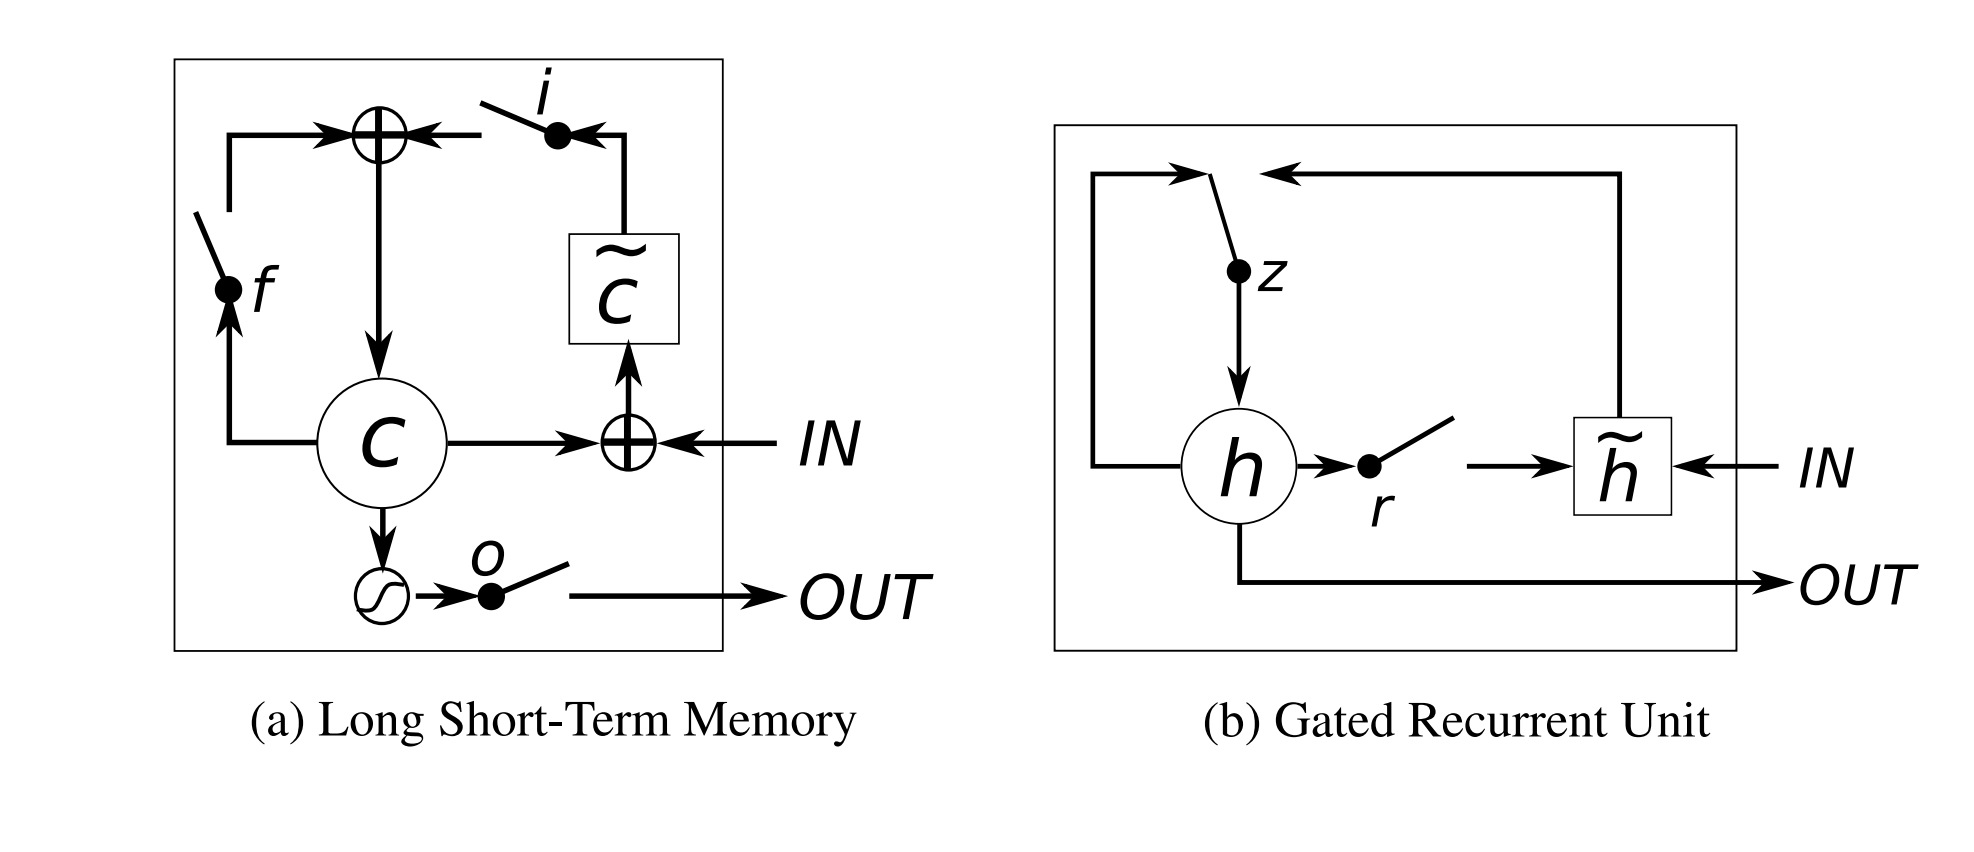
\includegraphics[scale = 0.2]{images/rnn.png}
    \caption{Illustration of (a) LSTM and (b) gated recurrent units. (a) i, f and o are the input, forget and output gates, respectively. c and \~c denote the memory cell and the new memory cell content. (b) r and z are the reset and update gates, and h and \~h are the activation and the candidate activation. Image and caption source: \cite{rnn}.}.
    \label{fig:rnn}
\end{figure}

\subsection{Deep Reinforcement Learning}

Deep RL refers to the use of neural networks within an RL algorithm to approximate some function. In the case of Q-learning in the previous section, a neural network can be used to approximate the state-action value function, $Q$. This modified algorithm is called deep Q-learning (DQN) \cite{dqn}.

In DQN, the neural network eliminates the need for storing a Q-table, significantly reducing the memory requirements. The neural network is better able to approximate state-action values that have not been seen before (but may be similar to those observed previously), allowing for better performance.

Experience replay \cite{expeirnecereplay} is the technique of storing the agent's experiences at each timestep ($e_t = (s_t, a_t, r_t, s_{t+1})$) in a dataset $D = e_1..., e_N$ called the replay memory \cite{dqn}.

As described in \cite{qmixcite}, the weights and biases of the network are learnt by sampling batches of the replay memory and minimising the \textit{TD error}:

\[\mathscr{L}(\theta)=\sum_{i=1}^{b}[(y_i^{DQN}-Q(s,a;\theta))^2]\]

where $y^{DQN}=r+\gamma \max_{a'}Q(s',a';\theta^-)$ ($\theta^-$ are the parameters for a \textit{target network} that are updated using $\theta$ periodically) \cite{qmixcite}.



\subsection{Multi-Agent Reinforcement Learning}
Multi-Agent Reinforcement Learning (MARL) is the process of learning policies for multiple co-operative (or adversarial) agents interacting in the same environment. In this project, we only consider co-operative agents. One paradigm of MARL is \textit{centralised learning with decentralised execution}, which allows for a single controller (which has access to the global state) to coordinate the learning of all agents, while during execution each agent operates independently using its learned policy.

\subsubsection{The StarCraft Multi-Agent Challenge}

Recent progress in MARL has seen the need for a benchmark of performance, including a specific environment and method for quantifying performance. A popular benchmark fitting this description is the StarCraft Multi-Agent Challenge (SMAC) \cite{smac}. SMAC is based upon the science-fiction real-time strategy game StarCraft II in which teams of various units battle against one another. Although the game is far more complex than this (with resource management, buildings as well as other considerations), SMAC only considers situations of this form. Each unit is controlled by a single agent, and SMAC specifies various maps (the number and type of the units on either team) as well as allowing control over the difficulty of the AI controlling the opposing team. 


In SMAC (and in this project) we consider the following unit types:

\vspace{3mm}
\begin{center}
\begin{tabular}{ |p{2.5cm}||p{6.6cm}|  }
 \hline
 \centering Unit Type& \centering Description \tabularnewline
 \hline
 \centering Marine   & A cheap, all-purpose infantry unit\tabularnewline
 \hline
 \centering Stalker   & A fast moving ranged unit\tabularnewline
 \hline
 \centering Zealot   &  A strong brute-force unit\tabularnewline
 \hline
 
\end{tabular}
\end{center}
\vspace{3mm}


\subsubsection{Dec-POMDPs}
A decentralised partially observable Markov decision process (dec-POMDP) is an extension of a regular MDP for use in multi-agent reinforcement learning. 

As described in \cite{dec-pomdp}, we can define a dec-POMDP as follows:
\begin{definition}\textbf{\normalfont{\cite{dec-pomdp}}}{ (Dec-POMDP)}
A decentralised partially observable Markov decision
process is defined as a tuple $\mathscr{M} = \langle \mathbb{D,S,A},T,\mathbb{O},O,R,b_0\rangle$, where
\begin{itemize}
    \item $\mathbb{D}=\{1,...,n\}$ is the set of n agents.
    \item $\mathbb{S}$ is a (finite) set of states.
    \item $\mathbb{A}$ is the set of joint actions.
    \item $T$ is the transition probability function.
    \item $\mathbb{O}$ is the set of joint observations.
    \item $O$ is the observation probability function.
    \item $R$ is the immediate reward function.
    \item $b_0$ is the initial state distribution at time $t = 0$.
    
\end{itemize}
\end{definition}

At each time step (with the environment in state $s \in \mathbb{S}$), each agent $d \in \mathbb{D}$ will choose an action $a^d$ (to form the joint action $\textbf{a} \in \mathbb{A}$) and will transition to a new state $s'$ with probability $T(s'|s,\textbf{a})$. Each agent will receive the reward $R(s, \textbf{a})$. Individual observations $o^d$ are made by each agent to form the joint observation $\textbf{o} \in \mathbb{O}$. A joint observation \textbf{o} occurs with probability $O(\textbf{o})$. There is an action-observation history $\tau^d \in (\mathbb{A} \times \mathbb{O})^*$ for each agent $d \in \mathbb{D}$. This conditions a stochastic policy $\pi^d(a^d|\tau^d) : (\mathbb{A} \times \mathbb{O})^* \times \mathbb{A} \to [0, 1]$. Intuitively, the policy $\pi^d$ gives the probability that a particular action $a^d$ is taken, given an action-observation history $\tau^d$, for agent $d$.

\subsubsection{Independent Q-Learning}
Independent Q-learning \cite{IQL} is a simple extension of Q-learning to the multi-agent setting. The problem is decomposed into multiple agents, each employing Q-learning independently, sharing the same environment. Although this technique does not account for the non-stationarity of sharing the same environment, it is surprisingly effective in practise \cite{iqlisgood}. 


\subsubsection{Value Decomposition Networks}
Value Decomposition Networks \cite{vdn} (VDN), by contrast, aim to learn a joint action-value function

\[Q_{tot}(\boldsymbol{\tau}, \textbf{a}) = \sum_{i=1}^{n} Q_i(\tau^i,a^i;\theta^i) \]

where $\boldsymbol{\tau}$ is the joint observation history, $\textbf{a}$ is the joint action, $Q_i$ is the utility function for agent $i$ and $\theta^i$ are the parameters for agent $i$'s network.

Q is then learnt in the same way as DQN, but during execution this policy is very easy to decentralise (each agent chooses greedily with respect to its own $Q_i$).

This follows the \textit{centralised learning with decentralised execution} paradigm.

\subsubsection{QMIX}
QMIX is a state-of-the-art deep MARL algorithm that lies between the extremes of IQL and centralised Q-learning \cite{qmixcite}. Instead of requiring the decentralised policies be consistent with the centralised counterpart, as in VDN, all that we require in this section is that a global argmax performed on $Q_{tot}$ yields
the same result as a set of individual argmax operations
performed on each $Q_a$:

\[\argmax_{\textbf{a}}Q_{tot}(\boldsymbol{\tau},\textbf{a}) = \begin{bmatrix}
        \argmax_{a^1}Q_1(\tau^1,a^1) \\
        \vdots\\
        \argmax_{a^n}Q_n(\tau^n,a^n)
    \end{bmatrix}\]







QMIX represents $Q_{tot}$ using an architecture
consisting of agent networks, a mixing network, and a set
of hypernetworks \cite{hypernetworks} \cite{qmixcite}. Each agent has its own deep recurrent Q-network (DRQN) \cite{dqrn},the outputs of which are fed into the mixing network: a feed-forward neural network that mixes them
monotonically, producing the values of $Q_{tot}$ \cite{qmixcite}. The weights of the mixing network are produced by separate hypernetworks \cite{qmixcite}.

An overview of the networks can be seen in figure \ref{fig:qmix}, but further details can be found in \cite{qmixcite}.

\begin{figure}
    \centering
    \hbox{\hspace{-2.5em}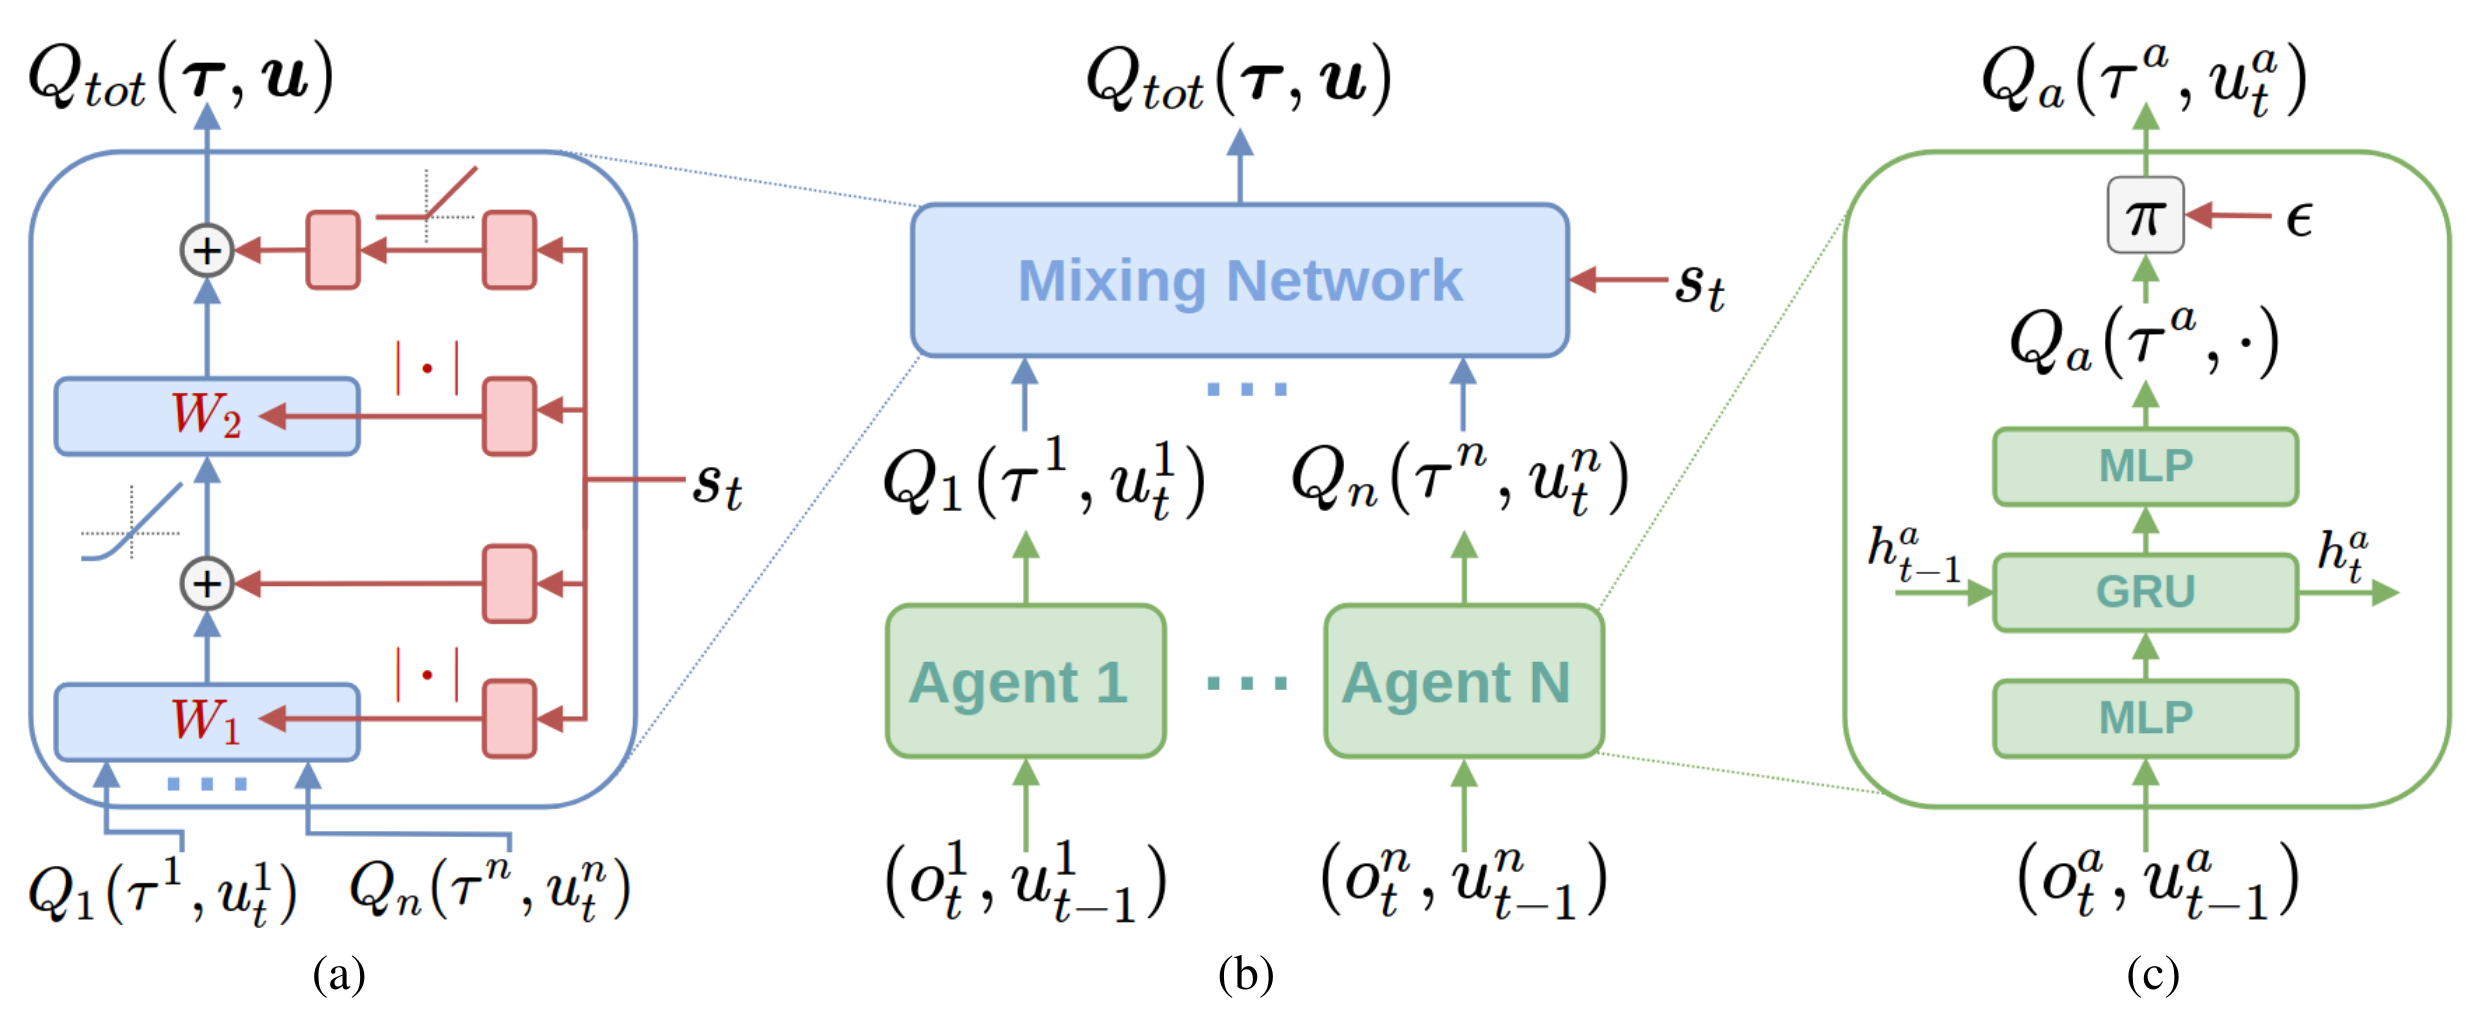
\includegraphics[scale = 0.18]{images/qmix.png}}
    \caption{(a) Mixing network structure. In red are the hypernetworks that produce the weights and biases for mixing network layers shown
in blue. (b) The overall QMIX architecture. (c) Agent network structure. Image and caption source: \cite{qmixcite}.}
    \label{fig:qmix}
\end{figure}





QMIX is trained in the same way as in DQN, replacing $Q$ with $Q_{tot}$.

